%%%%%%%%%%%%%%%%%%%%%%%%%%%%%%%%%%%%%%%%%%%%%%%%
% Python Cheat Sheet
% baposter Landscape Poster
% LaTeX Template
% Version 1.0 (11/06/13)
% baposter Class Created by:
% Brian Amberg (baposter@brian-amberg.de)
% This template has been downloaded from:
% http://www.LaTeXTemplates.com
% License:
% CC BY-NC-SA 3.0 (http://creativecommons.org/licenses/by-nc-sa/3.0/)
% Edited by Michelle Cristina de Sousa Baltazar
%%%%%%%%%%%%%%%%%%%%%%%%%%%%%%%%%%%%%%%%%%%%%%%%

%----------------------------------------------------------------
%	PACKAGES AND OTHER DOCUMENT CONFIGURATIONS
%----------------------------------------------------------------

\documentclass[landscape,a0paper,fontscale=0.285]{baposter} % Adjust the font scale/size here
\title{epib607 cheat sheet}
\usepackage[brazilian]{babel}
\usepackage[utf8]{inputenc}

\usepackage{graphicx} % Required for including images
%\graphicspath{{figures/}} % Directory in which figures are stored

\usepackage{xcolor}
\usepackage{colortbl}
\usepackage{tabu}
\usepackage{comment}
\usepackage{pifont}% http://ctan.org/pkg/pifont
\newcommand{\cmark}{\ding{51}}%
\newcommand{\xmark}{\ding{55}}%

\usepackage{mathtools}
%\usepackage{amsmath} % For typesetting math
\usepackage{amssymb} % Adds new symbols to be used in math mode

\usepackage{booktabs} % Top and bottom rules for tables
\usepackage{enumitem} % Used to reduce itemize/enumerate spacing
\usepackage{palatino} % Use the Palatino font
\usepackage[font=small,labelfont=bf]{caption} % Required for specifying captions to tables and figures

\usepackage{multicol} % Required for multiple columns
\setlength{\columnsep}{1.5em} % Slightly increase the space between columns
\setlength{\columnseprule}{0mm} % No horizontal rule between columns

\usepackage{tikz} % Required for flow chart
\usetikzlibrary{decorations.pathmorphing}
\usetikzlibrary{shapes,arrows} % Tikz libraries required for the flow chart in the template

\newcommand{\compresslist}{ % Define a command to reduce spacing within itemize/enumerate environments, this is used right after \begin{itemize} or \begin{enumerate}
\setlength{\itemsep}{1pt}
\setlength{\parskip}{0pt}
\setlength{\parsep}{0pt}
}

\definecolor{lightblue}{rgb}{0.145,0.6666,1} % Defines the color used for content box headers

\begin{document}

\begin{poster}
{
headerborder=closed, % Adds a border around the header of content boxes
colspacing=0.8em, % Column spacing
bgColorOne=white, % Background color for the gradient on the left side of the poster
bgColorTwo=white, % Background color for the gradient on the right side of the poster
borderColor=lightblue, % Border color
headerColorOne=black, % Background color for the header in the content boxes (left side)
headerColorTwo=lightblue, % Background color for the header in the content boxes (right side)
headerFontColor=white, % Text color for the header text in the content boxes
boxColorOne=white, % Background color of the content boxes
textborder=roundedleft, % Format of the border around content boxes, can be: none, bars, coils, triangles, rectangle, rounded, roundedsmall, roundedright or faded
eyecatcher=true, % Set to false for ignoring the left logo in the title and move the title left
headerheight=0.1\textheight, % Height of the header
headershape=roundedright, % Specify the rounded corner in the content box headers, can be: rectangle, small-rounded, roundedright, roundedleft or rounded
headerfont=\Large\bf\textsc, % Large, bold and sans serif font in the headers of content boxes
%textfont={\setlength{\parindent}{1.5em}}, % Uncomment for paragraph indentation
linewidth=2pt % Width of the border lines around content boxes
}
%----------------------------------------------------------------
%	TÍTULO
%----------------------------------------------------------------
{\bf\textsc{EPIB607 Cheat Sheet}\vspace{0.5em}} % Poster title
{\textsc{\{ E P I B 6 0 7 \ \ \ \ \ C h e a t \ \ \ \ \ S h e e t\} \hspace{12pt}}}
{\textsc{Sahir Rai Bhatnagar\\ (McGill University) \hspace{12pt}}} 


%------------------------------------------------
% Data Viz
%------------------------------------------------
\headerbox{Data Visualization}{name=objectives,column=0,row=0,span=2}{

%--------------------------------------
%\colorbox[HTML]{CCFFFF}{\makebox[\textwidth-2\fboxsep][l]{\bf - Dicas:}}
\begin{itemize}\compresslist
\item Commonly used aesthetics in data visualization: position, shape, size, color, line width, line type. Some of these aesthetics can represent both continuous and discrete data (position, size, line width, color) while others can only represent discrete data (shape, line type)
\item Cynthia Brewer palettes: Sequential, Diverging, Qualitative
\end{itemize}

\centering
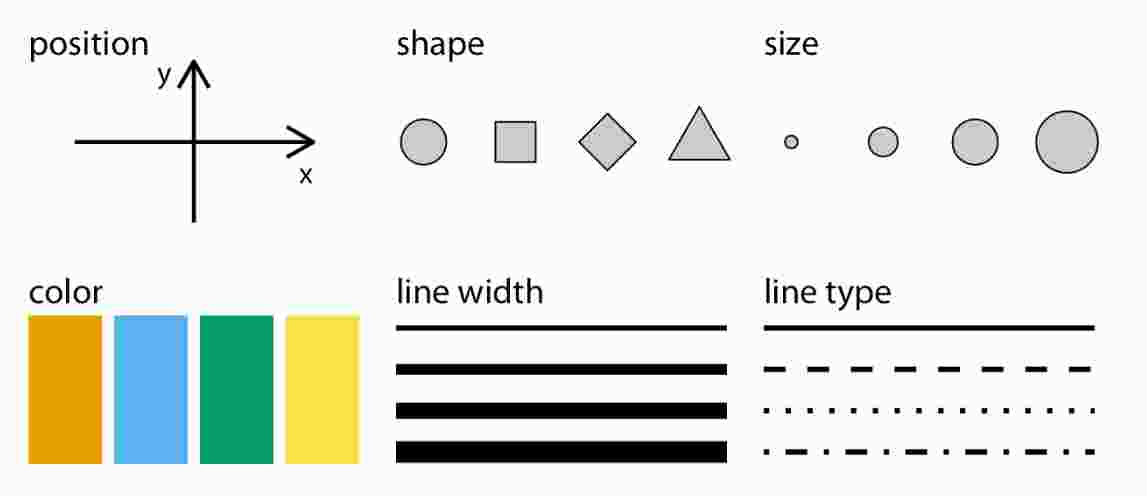
\includegraphics[scale=0.2]{scales.jpg}

\vspace{0.0em} % When there are two boxes, some whitespace may need to be added if the one on the right has more content
}


%------------------------------------------------
% Sampling Distributions, CLT, Confidence Intervals and p-values
%------------------------------------------------
\headerbox{Sampling Distributions, CLT, CI, p-value}{name=objectives,column=0,row=0.33,span=2}{

%--------------------------------------
%\colorbox[HTML]{CCFFFF}{\makebox[\textwidth-2\fboxsep][l]{\bf - Dicas:}}
\begin{itemize}\compresslist
\item \textbf{Standard error (SE)} of the sample mean is $\sigma/\sqrt{n}$
\item \textbf{SE($\bar{y}$)} describes how far $\bar{y}$ could (typically) deviate from $\mu$
\item \textbf{SD($y$)} describes how far an individual $y$ (typically) deviates from $\mu$ (or from $\bar{y}$).
\end{itemize}
\begin{itemize}\compresslist
	\item \textbf{Paramter}: An  unknown  numerical  constant  pertaining  to  a  population/universe,  or  in  a  statistical  model. $\mu$: population mean, $\pi$: population proportion, $\lambda$: population rate
	\item \textbf{Statistic}: A  numerical  quantity  calculated  from  a  sample. The  empirical counterpart of the parameter,  used  to  \textit{estimate}  it. $\bar{y}$: sample mean, $p$: sample proportion, $\hat{\lambda}$: sample rate
\end{itemize}
	\begin{itemize}\compresslist
		\item \textbf{Sampling Distribution} of a statistic is the distribution of values taken by the statistic in all possible samples of the same size from the same population. The standard deviation of a sampling distribution is called a standard error.
	\end{itemize} 


\vspace{0.0em} % When there are two boxes, some whitespace may need to be added if the one on the right has more content
}

%------------------------------------------------
% One sample mean
%------------------------------------------------
\headerbox{One sample mean}{name=objectives,column=0,row=0.64,span=2}{
\begin{center}
	\begin{tabular}{|l|c|c|} \hline
		$\sigma$& known & unknown \\ \hline Data & $\{y_1,y_2,...,y_n\}$ &
		$\{y_1,y_2,...,y_n\}$\\
		& & \\
		Pop'n param & $\mu$ & $\mu$\\
		& & \\
		Estimator & $\overline{y} = \frac{1}{n}\sum_{i=1}^n y_i$ & $\overline{y} = \frac{1}{n}\sum_{i=1}^n y_i$ \\
		& & \\
		SD & $\sigma$ & $s = \sqrt{\frac{\sum_{i=1}^n(y_i-\overline{y})^2}{n-1}}$ \\
		& & \\
		SEM & $\sigma/\sqrt{n}$ & $s / \sqrt{n}$ \\
		& & \\
		$(1-\alpha)100$\% CI & $\overline{y} \pm z^\star_{1-\alpha/2}$(SEM) & $\overline{y} \pm t^\star_{1-\alpha/2, (n-1)}$(SEM) \\
		& & \\
		test statistic & $\frac{\overline{y}-\mu_0}{\textrm{SEM}}\sim \mathcal{N}(0,1)$ &
		$\frac{\overline{y}-\mu_0}{\textrm{SEM}}\sim t_{(n-1)}$ \\
		\hline
	\end{tabular}
\end{center}
}

%------------------------------------------------
% Assumptions
%------------------------------------------------
\headerbox{Assumptions}{name=objectives,column=2,row=0.60,span=2}{
\begin{center}
	\begin{tabular}{|l|c|c|c|} \hline
		& $z$ & $t$ & Bootstrap \\ 
		\hline 
		SRS & \cmark &\cmark &	\cmark\\
		& & & \\
		Normal population & \cmark$^\star$ & \cmark$^\star$ &  \xmark\\
		& & &\\
		needs CLT &  \cmark$^\star$ & \cmark$^\star$ &  \xmark\\
		& & &\\
		$\sigma$ known  & \cmark & \xmark & \xmark\\
		& & &\\
		Sampling dist. center at & $\mu$ & $\mu$ & $\bar{y}$\\
		& & &\\
		SD & $\sigma$ & $s$ & $s$ \\
		& & &\\
		SEM & $\sigma/\sqrt{n}$ & $s / \sqrt{n}$ & SD(bootstrap statistics) \\
		\hline
	\end{tabular}

\footnotetext[1]{*If population is Normal then CLT is not needed. If population is not Normal then CLT is needed.}
\end{center}
}



%------------------------------------------------
% Lógica Básica do Python
%------------------------------------------------

\begin{comment}
\headerbox{Lógica Básica do Python}{name=introduction,column=1,row=0,bottomaligned=objectives}{

%------IF--------
\colorbox[HTML]{CCFFFF}{\makebox[\textwidth-2\fboxsep][l]{\bf - if}}
\begin{itemize}\compresslist
\item if teste:\\
........\# faça algo se teste der verdadeiro\\
elif teste2\\
........\# faça algo se teste2 der verdadeiro\\
else:\newline
........\# faça algo se ambos derem falso
\end{itemize}


%------WHILE--------
\colorbox[HTML]{CCFFFF}{\makebox[\textwidth-2\fboxsep][l]{\bf - while:}}
\begin{itemize}\compresslist
\item while teste:\\
........\# enquanto verdadeiro continue fazendo algo
\end{itemize}


%------FOR--------
\colorbox[HTML]{CCFFFF}{\makebox[\textwidth-2\fboxsep][l]{\bf - for:}}
\begin{itemize}\compresslist
\item for x in sequência\\
........\# enquanto o x estiver na sequência informada\\
........\# faça algo para cada item na sequência\\
........\# a sequência pode ser uma lista,\\
........\# elementos de uma string, etc.

\item for x in range(10)\\
........\# repita algo 10 vezes (de 0 a 9)

\item for x in range(5,10)\\
........\# repita algo 5 vezes (de 5 a 9)
\end{itemize}

\colorbox[HTML]{CCFFFF}{\makebox[\textwidth-2\fboxsep][l]{\bf - Testes Lógicos}}
\linebreak \\
\begin{tabular}{l l}
10 == 10 & retorna: True \\
10 == 11 & retorna: False \\
10!= 11 & retorna: True \\
"jack" == "jack" & retorna: True \\
"jack" == "jake" & retorna: False \\
10 > 10 & retorna: False \\
10 >= 10 & retorna: True \\
"abc" >= "abc" & retorna: True \\
"abc" < "abc" & retorna: False \\
\end{tabular}
\end{comment}


%------------------------------------------------
% R Code
%------------------------------------------------

\headerbox{R Code}{name=results,column=2,span=2,row=0}{

%\colorbox[HTML]{CCFFFF}{\makebox[\textwidth-2\fboxsep][l]{\bf - Listas no Python}}
%\linebreak \\
%Listas são compostas por elementos de qualquer tipo (podem ser alteradas) \linebreak \\
\begin{tabular}{@{}ll@{}}
\textbf{Normal Distribution} $Y\sim \mathcal{N}(\mu, \sigma^2)$\\
\multicolumn{2}{l}{\cellcolor[HTML]{DDFFFF} Cumulative Probabilities: \texttt{pnorm(q = , mean = , sd = , lower.tail = TRUE)}} \\
\multicolumn{2}{l}{\cellcolor[HTML]{FFFFFF} Quantiles: \texttt{qnorm(p = , mean = , sd = )}} \\
\multicolumn{2}{l}{\cellcolor[HTML]{DDFFFF} Linear regression: \texttt{lm(y $\sim$ x, data = df)}} \\ 
\multicolumn{2}{l}{\cellcolor[HTML]{DDFFFF} log link $\to$: \texttt{glm(y $\sim$ x, data = df, family=gaussian(link="log"))}} \\ \ \\
\end{tabular}
%------------------------------------------------

\begin{tabular}{@{}ll@{}}
\textbf{t Distribution} $Y\sim t_{(df)}$\\
\multicolumn{2}{l}{\cellcolor[HTML]{DDFFFF} Cumulative Probabilities: \texttt{pt(q = , df = , lower.tail = TRUE)}} \\
\multicolumn{2}{l}{\cellcolor[HTML]{FFFFFF} Quantiles: \texttt{qt(p = , df = )}} \\ \ \\
\end{tabular}

%------------------------------------------------

\begin{tabular}{@{}ll@{}}
\textbf{Binomial Distribution} $Y\sim Binomial(N, \pi)$\\
\multicolumn{2}{l}{\cellcolor[HTML]{DDFFFF} Cumulative Probabilities $P(Y \leq k)$: \texttt{pbinom(q=,size=,prob=,lower.tail=TRUE)}} \\
\multicolumn{2}{l}{\cellcolor[HTML]{DDFFFF} Cumulative Probabilities $P(Y > k)$: \texttt{pbinom(q=,size=, prob=,lower.tail=FALSE)}} \\
\multicolumn{2}{l}{\cellcolor[HTML]{FFFFFF} Quantiles: \texttt{qbinom(p = , size = , prob = )}} \\
\multicolumn{2}{l}{\cellcolor[HTML]{DDFFFF} Probabilities $P(Y=k)$: \texttt{dbinom(x = ,size = ,prob = )}} \\
\multicolumn{2}{l}{\cellcolor[HTML]{FFFFFF} Logistic regression: \texttt{glm(y $\sim$ x, data = df, family = binomial(link="logit"))}} \\ 
\multicolumn{2}{l}{\cellcolor[HTML]{FFFFFF} log link $\to$: \texttt{glm(y $\sim$ x, data = df, family = binomial(link="log"))}} \\ \ \\
\end{tabular}

%------------------------------------------------

\begin{tabular}{@{}ll@{}}
\textbf{Poisson Distribution} $Y\sim Poisson(\lambda)$\\
\multicolumn{2}{l}{\cellcolor[HTML]{DDFFFF} Cumulative Probabilities $P(Y \leq k)$: \texttt{ppois(q = , lambda = , lower.tail=TRUE)}} \\
\multicolumn{2}{l}{\cellcolor[HTML]{DDFFFF} Cumulative Probabilities $P(Y > k)$: \texttt{ppois(q = , lambda =, lower.tail=FALSE)}} \\
\multicolumn{2}{l}{\cellcolor[HTML]{FFFFFF} Quantiles: \texttt{qpois(p = , size = , prob = )}} \\
\multicolumn{2}{l}{\cellcolor[HTML]{DDFFFF} Probabilities $P(Y=k)$: \texttt{dpois(x = ,lambda = )}} \\
\multicolumn{2}{l}{\cellcolor[HTML]{FFFFFF} Poisson regression: \texttt{glm(y$\sim$x+offset(log(PT)),data=df,family=poisson(link="log"))}}  \\
\multicolumn{2}{l}{\cellcolor[HTML]{FFFFFF} identity link: \texttt{glm(y $\sim$ -1 + PT + PT:x,family=poisson(link="identity"))}}  \\
\end{tabular}


}
\end{poster}


\end{document}

\newpage

%%%%%%%%%%%%%%%%%%%%%%%%%%%%%%%%%%%%%%%%%%%%%%%%%%%%%%%%%%
%%%%%%%%%%%%%%%%%%    SEGUNDA PÁGINA    %%%%%%%%%%%%%%%%%%
%%%%%%%%%%%%%%%%%%%%%%%%%%%%%%%%%%%%%%%%%%%%%%%%%%%%%%%%%%

\begin{poster}
{
headerborder=closed, colspacing=0.8em, bgColorOne=white, bgColorTwo=white, borderColor=lightblue, headerColorOne=black, headerColorTwo=lightblue, 
headerFontColor=white, boxColorOne=white, textborder=roundedleft, eyecatcher=true, headerheight=0.1\textheight, headershape=roundedright, headerfont=\Large\bf\textsc, linewidth=2pt 
}
%----------------------------------------------------------------
%	TITLE SECTION 
%----------------------------------------------------------------
{\bf\textsc{Python Cheat Sheet}\vspace{0.5em}} % Poster title
{\textsc{\{ P y t h o n \ \ \ \ \ C h e a t \ \ \ \ \ S h e e t\} \hspace{12pt}}}
{\textsc{Michelle Cristina de Sousa Baltazar \\ (Universidade Federal do Triângulo Mineiro) \hspace{12pt}}} 

%----------------------------------------------------------------
%	Outros Elementos
%----------------------------------------------------------------
\headerbox{Outros Elementos}{name=method,column=0}{

\colorbox[HTML]{CCFFFF}{\makebox[\textwidth-2\fboxsep][l]{\bf - Palavras-Chave}}
\begin{tabular}{lp{5.8cm}lp{1.0cm}}
{\bf Oper.} & {\bf Descrição}\\
print & Imprime para a tela \\
while & "Enquanto" - laço para repetição de alguma condição \\
for & "Para" - loop para repetição de alguma condição \\
break & Interrompe o loop caso necessário \\
continue & Interrompe o loop atual sem sair do loop, reiniciando \\
if & "Se" - usado para testar alguma condição \\
elif & É uma variante para o "senão" - se a primeira condição falha, testa a próxima \\
else & "Senão" - é opicional e será executado quando a primeira condição falhar \\
is & Testa a identidade do objeto \\
import & Importa outros módulos para dentro de um script \\
as & Usado para dar um apelido (alias) para um módulo \\
from & Para importar uma variável especifica, classe ou função de um módulo \\
def & Usado para criar uma função nova definida pelo usuário \\
return & Sai da função e retorna um valor \\
lambda & Cria uma função nova anônima \\
global & Acessa variáveis definida globalmente (fora de uma função) \\
try & Especifica manipuladores de exceções  \\
except & Captura a exceção e executa códigos \\
finally & É sempre executado no final, utilizado para limpar os recursos \\
raise & Cria uma exceção definida pelo usuário \\
del & Deleta objetos \\
pass & Não faz nada \\
assert & Usado para fins de depuração \\
class & Usado para criar objetos definidos pelo usuário \\
exec & Executa dinamicamente um código Python \\
yield & É usado com geradores
\end{tabular}


}

%----------------------------------------------------------------
%	Operadores
%----------------------------------------------------------------
\headerbox{Operadores Python}{name=results2,column=1}{
Tomemos como exemplo a=10 e b=20:\\
\colorbox[HTML]{CCFFFF}{\makebox[\textwidth-2\fboxsep][l]{\bf - Operadores Aritméticos}}
\begin{tabular}{lll}
{\bf Op.} & {\bf Descrição} & {\bf Exemplo} \\
+ & Adição & a + b retorna: 30 \\
- & Subtração & a - b retorna: -10 \\
* & Multiplicação & a * b retorna: 200 \\
/ & Divisão & b / a retorna: 2 \\
\% & Módulo & a \% b retorna: 0 \\
** & Exponencial & a**b retorna: $10^{20}$ \\
// & Divisão Piso & 9 // 2 retorna: 4
\end{tabular}

%----OPERADORES DE COMPARAÇÃO-----------
\colorbox[HTML]{CCFFFF}{\makebox[\textwidth-2\fboxsep][l]{\bf - Operadores de Comparação}}
As operações básicas de comparação podem ser usadas de diversas maneiras para todos os tipos de valores - números, strings, sequencias, listas, etc. O retorno será sempre True ou False.\\
\begin{tabular}{lll}
{\bf Op.} & {\bf Descrição} & {\bf Exemplo} \\
< & Menor que & a < b retorna: True \\
<= & Menor ou igual & a <= b retorna: True \\
== & Igual & a == b retorna: False \\
> & Maior que & a > b retorna: False \\
>= & Maior ou igual & a >= b retorna: False \\
!= & Diferente & a != b retorna: True \\
<> & Diferente & a <> b retorna: True
\end{tabular}

%------OPERADORES LÓGICOS-----------
\colorbox[HTML]{CCFFFF}{\makebox[\textwidth-2\fboxsep][l]{\bf - Operadores Lógicos}}
Os operadores lógicos {\bf and} e {\bf or} Também retornam um valor booleano quando usado em uma estrutura de decisão.\\
\begin{tabular}{lp{6.5cm}lp{1.0cm}|}
{\bf Op.} & {\bf Descrição}\\
and & Se o resultado de ambos operadores é verdadeiro, retorna: True \\
or & Se um dos resultados retorna verdadeiro, retorna: True \\
not & É utilizado para reverter o estado lógico de qualquer operação booleana.
\end{tabular}

%-------TUPLAS---------------------
\colorbox[HTML]{CCFFFF}{\makebox[\textwidth-2\fboxsep][l]{\bf - Tuplas no Python}}
Tupla é uma lista de valores separados por vírgulas - é similar à uma lista porém é imutável: \\ 
uma\_tupla = 'a','b','c','d','e' \\
outra\_tupla = ('a','b','c','d','e') \\

%------NÚMEROS ALEATÓRIOS----------
\colorbox[HTML]{CCFFFF}{\makebox[\textwidth-2\fboxsep][l]{\bf - Números Aleatórios}}
Strings são compostos de caracteres: \\ 
uma\_string = "Hello World!" \\
outra\_string = 'Ola Mundo!"

}

%----------------------------------------------------------------
%	Strings no Python
%----------------------------------------------------------------
\headerbox{Strings no Python}{name=conclusion,column=2,span=2,row=0}{
string é uma sequencia de caracteres geralmente usada para armazenar texto. \\
Strings são compostos de caracteres (não podem ser alterados - são imutáveis) \\ 
\linebreak
%% {lp{5.8cm}lp{1.0cm}|}
\begin{tabular}{@{}lp{10.2cm}l@{}}
\multicolumn{2}{l}{\cellcolor[HTML]{DDFFFF}Criação} \\
uma\_string = "Hello World!" & outra\_string = 'Ola Mundo!" \\
\multicolumn{2}{l}{\cellcolor[HTML]{DDFFFF}Acessando} \\
uma\_string[4] & retorna: 'o' \\
\multicolumn{2}{l}{(este caso retorna a 4ª posição do texto - começando a contar a partir do zero)} \\
\multicolumn{2}{l}{\cellcolor[HTML]{DDFFFF}Dividindo} \\
uma\_string.split('') & retorna ['Hello','World'] \\
\multicolumn{2}{l}{(este caso divide o texto no espaço em branco em uma lista de duas strings)} \\
uma\_string.split('r') & retorna ['Hello Wo','ld'] \\
\multicolumn{2}{l}{(este caso divide o texto na letra 'r' em uma lista de duas strings)} \\
\multicolumn{2}{l}{\cellcolor[HTML]{DDFFFF}Unindo} \\
\multicolumn{2}{l}{Para unir uma lista de strings usaremos a função join() } \\
\multicolumn{2}{l}{uma\_lista = ["isto","eh","uma","lista","de","strings"]} \\
' '.join(uma\_lista) & retorna: "isto eh uma lista de strings" \\
' 'TESTE'.join(uma\_lista) & Retorna: \\
''.join(uma\_lista) & retorna: "istoehumalistadestrings" \\
\multicolumn{2}{l}{\cellcolor[HTML]{DDFFFF}Formatando Strings} \\
\multicolumn{2}{l}{Podemos usar o operador \% para adicionar elementos em uma string:} \\
\multicolumn{2}{l}{esta\_string = "todos"} \\
print("Olá para \%s!" \%esta\_string) & retorna: "Olá para todos!" \\
\end{tabular}
\linebreak

%-----OPERAÇÕES COM STRINGS----------
\colorbox[HTML]{CCFFFF}{\makebox[\textwidth-2\fboxsep][l]{\bf - Operações com Strings}}
Definindo as variaveis de string para exemplo da seguinte forma: a = ['Hello'] e b = ['Python'] \\
\begin{tabular}{lp{9.0cm}lp{1.0cm}lp{1.0cm}} %\begin{tabular}{lll}
{\bf Oper.} & {\bf Descrição} & {\bf Exemplo} \\
+ & Concatenation - soma o conteúdo das duas strings & a + b retorna: HelloPython \\
* & Repetition - repete o conteúdo da string N vezes & a*2 retorna: HelloHello \\
.[ ] & Slice - fatia retornando o caractere no respectivo indice & a[1] retorna: "e" \\
.[ : ] & Range Slice - retorna os caracteres do intervalo indicado & a[1:4] retorna: "ell" \\
in & Membership - se o caractere existe na string, retorna true & H in a will give 1 \\
not in & Membership - se o caractere não existe na string, retorna true & M not in a retorna: 1 \\
\% & Format - formata uma string & exemplos na tabela seguinte \\
\end{tabular}

%------FORMATAÇÃO DE STRINGS---------
\colorbox[HTML]{CCFFFF}{\makebox[\textwidth-2\fboxsep][l]{\bf - Formatação de Strings}}
\begin{tabular}{ll|ll} %\begin{tabular}{lp{3.0cm}lp{4.0cm}lp{2.0cm}lp{2.0cm}|} 
{\bf Símbolo} & {\bf Conversão} & {\bf Símbolo} & {\bf Conversão} \\
\%c & caractere					& \%i & decimal inteiro com sinal \\
\%d & decimal inteiro com sinal	& \%u & decimal inteiro sem sinal \\
\%o & octal inteiro				& \%x & hexadecimal inteiro (letras minúsculas) \\
\%f & numero real ponto flutuante & \%X & hexadecimal inteiro (letras maiúsculas) \\
\%g & o menor entre \%f e \%e & \%e & notação exponencial (com 'e' minúsculo) \\
\%G & o menor entre \%f e \%E & \%E & notação exponencial (com 'E' maiúsculo) \\
. & . & \%s & converção de string via str() antes de formatar \\
\end{tabular}

%-----------------------------------
}
%----------------------------------------------------------------
%	REFERENCES  {name=objectives,column=0,row=0}
%----------------------------------------------------------------
%\headerbox{bb}{name=references,column=1,row=0}{}
%----------------------------------------------------------------
%	FUTURE RESEARCH
%----------------------------------------------------------------
%\headerbox{aa}{name=futureresearch,column=1,row=0}{}
%----------------------------------------------------------------
%	CONTACT INFORMATION
%----------------------------------------------------------------
%\headerbox{Contact Information}{name=contact,column=2,span=2,row=0}{}
%----------------------------------------------------------------
\end{poster}
\end{document}